\chapter{Literature Review}\label{ch:litRev}

  The following literature review comprises of a systematic study of the current state of technology and systems in place that are relevant to the thesis. The two main components required to successful achieve the aim are: 
  \begin{enumerate}
      \item Develop a real time indoor positioning system to track the patient in the hospital out-patient environment.
      \item Determine areas which have a high risk of cross infection based on SNA of the mobility data collected from the RTLS.
  \end{enumerate}  
  A systematic and structured method, inspired by the guidelines of \citeauthor{webster2002analyzing} \cite{webster2002analyzing}, was followed to perform this review.
    
    Firstly, we will look into current RTLS implementations used in hospital environments. Secondly, we will review indoor positioning technologies making use of smart-phones presented in literature. This analysis will serve as a basis for the design of the real time patient positioning system. Finally, research will be conducted on the used of SNA in infection control.
    
    	\section{RTLS in Health Care} \label{ssec:litRev_RTLShospital}
        
        % what are the current systems used in hospitals
        % what is mobility data used for in hospital environments?
        
        It is apparent from \citeauthor{orwat2008towards} \cite{orwat2008towards} that technology has become an integral component of the health care industry, stating that computing has "entered health care in almost every setting". In specific, RTLS in health care is used for multiple applications as demonstrated by \citeauthor{boulos2012real} \cite{boulos2012real}. The common technologies used in RTLS consists of specialised fixed receivers or readers (location sensors) receiving wireless signals from small ID badges or tags attached to objects of interest and/or persons, to determine where the tagged entities are located within a building or some other confined indoor or outdoor space \cite{boulos2012real}. This is shown in Figure \ref{fig:litRev_RTLS_healthcare}.
        
        \begin{figure} [ht!]
        	\centering	
			\fbox{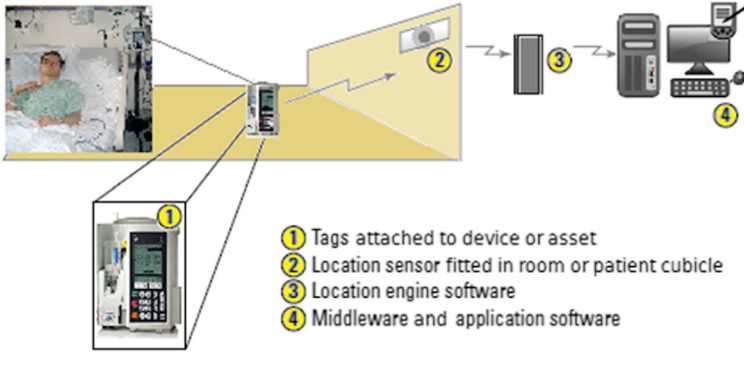
\includegraphics[scale=0.4]{RTLS_healthcare}}
            \caption{RTLS components in health care \cite{boulos2012real}}
            \label{fig:litRev_RTLS_healthcare}
		\end{figure}
        
        % applications of RTLS
        RTLS are currently deployed to help protect patients and staff by monitoring movement of patients, staff, visitors and equipment in real time to detect instantly their whereabouts and analyse historical movement \cite{cobbley2011easing}. The applications also extend to improving work flow. Tracking patient flows for throughput management can help diagnose bottlenecks and tailor appropriate solutions for problems such as extended waiting times, overcrowding and boarding in outpatient clinics, emergency departments/rooms (ED/ER); bumped and late surgeries; and the lack of available routine inpatient and intensive care unit (ICU) beds \cite{boulos2012real,stahl2011measuring,drazen2011using,malik2009rtls}.
        
        % impact of RTLS 
        The impact of RTLS systems have been significant in the health care industry. \citeauthor{laskowski2012rtls} \cite{laskowski2012rtls} and \citeauthor{boulos2012real} in \cite{boulos2012real} report impressive RTLS-enabled workflow efficiencies, including quantifiable significant cuttings in ED wait times, length of stay (LOS) and `left without being seen' (LWBS) rates. The value of the intelligence gleaned from RTLS patient flow data can be maximised by combining it with `lean production system principles' (pioneered by Toyota Motor Corporation) to optimise patient flows \cite{boulos2012real}. Other benefits of patient flow tracking and optimisation include fewer ambulance diversions and higher patient satisfaction ratings \cite{drazen2011using}, which can translate into improving the care facility’s perception and reputation.
        
        % limitations of RTLS
        Although there are significant benefits, the choice of RTLS technology must be very carefully made. A given technology or hardware may not work well despite all its merits, if not properly matched to the intended application or the hospital environment, budget and future expansion plans (the latter will require an adequately scalable RTLS solution) \cite{boulos2012real}. For example, radio signals are susceptible to interference via signal propagation, metals, water, people, and radio. Not every environment is suited for RF (radio frequency) systems. 
        
        % limitations of RTLS relevant to our thesis
       One can conclude that RTLS systems are an emerging standard in hospital environments. However, their use is largely focused to locating and/or analysing the flow of the various `players' (patients, doctors, nurses, equipment) in the hospital environment. There has been no establishment of a clear link between RTLS systems in controlling the transmission of infections within the hospital environment. Furthermore, the use of RF technologies for localisations poses issues with accuracy and scalability (as discussed in Section \ref{ssec:litRev_indoor}). 
                
        \section{Indoor Positioning Technologies} \label{ssec:litRev_indoor}
        
        In outdoor localization contexts, the most well-known and widely spread technology is the Global Positioning System (GPS). It is able to guarantee excellent performance in outdoor scenarios but experiences issues in indoor environments due to poor satellite coverage and signal degradation. Thus, the use of indoor localization techniques is increasingly becoming an essential component for a large number of applications and contexts such as "healthcare, home-care, monitoring, tracking, etc" \cite{mainetti2014Indoorlit}. Currently, indoor localisation lacks a ubiquitous system comparative to GPS. This is due to: errors by multipath and Non-Line-of-Sight (NLoS) conditions, presence of moving people that modify the indoor propagation channel, greater density of obstacles that cause a high attenuation and signal scattering, demand of a higher precision and accuracy \cite{mainetti2014Indoorlit}.
        
        \citeauthor{fallah2013indoor} \cite{fallah2013indoor} have grouped indoor localisation methods into four different techniques:(a) dead-reckoning, (b) direct sensing, (c) triangulation, and (d) pattern-recognition. These methods are discussed in the sections below.
        
        	\subsection{Pedestrian Dead Reckoning}           
            % talk about DR methods and algorithms that can be implemented
            These systems use sensors on the user to estimate relative rather than absolute location i.e. the change in position since the last update. The sensors utilised can be can be a combination of sensors such as accelerometers, magnetometers, compasses, and gyroscopes \cite{fallah2013indoor} or using a user’s specific walking pattern (such as the user’s average walking speed) \cite{wu2007pathplan}. They require little or no infrastructure to be pre-installed in buildings, but without an external reference, errors quickly accrue \cite{harle2013PIndoor}. This accrued error can be corrected by synchronizing direct sensing localisation techniques however the drawbacks of the direct sensing mechanism (for example blue-tooth beacons) are also applied to the system \cite{fallah2013indoor}.
            
            Dead-reckoning for walking users and hybrid systems using such techniques are called Pedestrian Dead-Reckoning (PDR) systems. These systems are of particular importance because they retain the low deployment costs associated with dead-reckoning whilst successfully addressing many of the shortcomings \cite{harle2013PIndoor}. Furthermore,  a Step-and-Heading Systems (SHS) is specific to pedestrians, estimating position by accruing distance and heading vectors representing steps \cite{harle2013PIndoor}. The fundamental cycle for an SHS is:
            \begin{enumerate}
				\item identify subsets of the data corresponding to individual step;
                \item estimate the length of the step; and
                \item estimate the step heading or change in heading.
			\end{enumerate}
            
            \subsubsection{Step Detection}
            
            \begin{figure}[ht!]
                \centering        
                \fbox{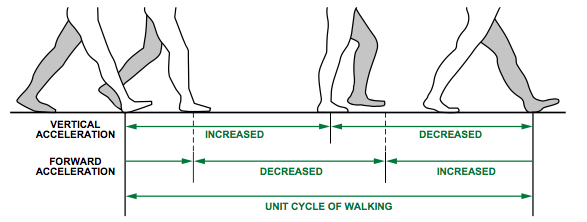
\includegraphics[scale=0.6]{stepMotion}}
                \caption{Walking Stages and Acceleration Pattern \cite{zhao2010full}}
                 \label{fig:litRev_stepMotion}
          	  \end{figure}
            
            Various techniques using accelerometer and gyroscope sensor data have been developed to detect the step motion. Figure \ref{fig:litRev_stepMotion} depicts a single step, defined as a unit cycle of walking behaviour, showing the relationship between each stage of the walking cycle and the change in vertical and forward acceleration. \citeauthor{harle2013PIndoor} has identified the following algorithms \cite{harle2013PIndoor}:
            \begin{enumerate}
            	\item \textbf{Peak Detection} - the heel strike is associated with sharp changes to the vertical acceleration. Standard peak detection algorithms can be used to highlight potential strikes. Note that each foot impact may generate multiple local peaks the nearer to the foot it is sited, due to the higher forces resulting in sensor bounce  \cite{ying2007automatic}. This can significantly increase the algorithm complexity.
               	\item \textbf{Zero Crossings} - is a method by which accelerometer readings are monitored for zero crossings \cite{goyal2011strap}.
                \item \textbf{Spectral analysis} - this involves computing the frequency spectrum of the cyclic data and identifying strong peaks at typical stepping frequencies. Subsets of the data (of a size that includes at least two cycles) are converted to the frequency domain and the dominant frequency taken as the walking frequency \cite{levi1996dead}.
			\end{enumerate}
            
            \subsubsection{Step Length Calculation}
            The simplest approach to estimating step length is to assign a constant value \cite{harle2013PIndoor}. However this approach can be too simplistic as \citeauthor{weinberg2002using}  reported that the step length can vary by as much as 40\% between pedestrians walking at the same speed, and up to 50\% across the range of walking speeds of an individual \cite{weinberg2002using}.
            
            \citeauthor{weinberg2002using} also described a dynamic step length estimation procedure based on the maximum vertical displacement of the hip (“bounce”). The stride length was shown to be a function of the bounce and the vertical angle between the highest and lowest point of the hip during a single stride \cite{weinberg2002using}. This angle is taken as constant although it is actually related to the leg length of the user. Nonetheless the step lengths are reported to be within 8\% of their true values.
            
            \subsubsection{Heading Estimation}
            
            Single integration of gyroscope signals provides estimates of heading change. Because SHSs can avoid using subsequent integration for the step length, the overall drift does at least grow linearly rather than cubically. In addition, some systems use only a single gyroscope mounted parallel to the torso, making the assumption that it remains (near) vertical during walking. Magnetometers may also be used directly or fused with the gyroscope outputs to estimate heading \cite{harle2013PIndoor}.
            
            \subsection{Direct Sensing}
             % RFIF, IR, Ultrasound, BT
             Direct sensing based localisation utilise the identifiers or tags to localise to a coordinate. Two approaches can be applied in the direct sensing method:  (a) location information and information on the user’s environment is stored in the tag itself; or (b) this information is retrieved from
a database using the tags’ unique identifier \cite{fallah2013indoor}.  The user’s orientation can be determined from relative changes in location from subsequent reads of tags \cite{willis2005rfid}.

			\citeauthor{fallah2013indoor} have identified these common direct sensing technologies:
            
            \begin{figure}[htbp!]
                \centering        
                \fbox{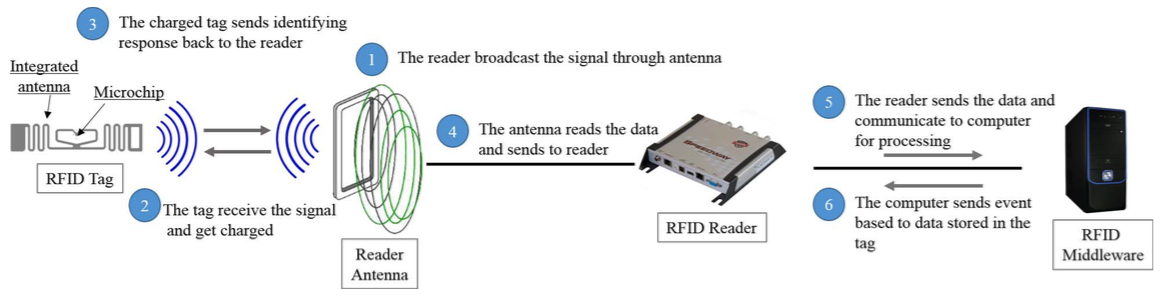
\includegraphics[scale=0.4]{RFIDschema}}
                \caption{A generalised RFID System\cite{mainetti2014Indoorlit}}
                 \label{fig:litRev_RFIDschema}
          	  	\end{figure}
              
            \begin{enumerate}
				\item \textbf{Infrared (IR)}: is one on the most common wireless technology used to localize objects or people through infrared emitters and receivers \cite{mainetti2014Indoorlit}. This technology can provide several advantages. First, IR beam does not penetrate through walls then it is possible to obtain a confinement of the signals inside the room \cite{mainetti2014Indoorlit}. Moreover, IR technology is characterized by the absence of radio electromagnetic interference and the power of transmitted IR signal can be easily adjusted to cover only the area of interest. Nevertheless, there are also several drawbacks. The multipath errors reduces drastically the localization accuracy and IR based indoor systems have expensive system hardware and maintenance costs. Furthermore, IR technology requires a Line of Sight (LoS) between transmitter and receiver to function properly \cite{mainetti2014Indoorlit}.
                
                \item \textbf{Radio Frequency Identifier Description (RFID)} : The RFID technology is based on the use of an RFID reader equipped with one or more reader antenna and active or passive transceivers (i.e., tags). The general system components are shows in Figure \ref{fig:litRev_RFIDschema}. The RFID technology works without direct LoS since the radio waves have the ability to penetrate solid materials, but strength of the signal depends upon the density of the objects in the building, and then accuracy is often limited \cite{mainetti2014Indoorlit}. In addition to the possibility to work in NLoS environment, other advantages of the RFID technology are high data rate, high security, cost effectiveness, and compactness. Main limitations of low frequency (125-134 kHz) and high frequency (13.56 MHz) RFID technology are related to a short reading range and to the ability to read only a few tags at the same time.         
                \item \textbf{Ultrasound identification (USID) }: use ultrasonic waves to measure distance between fixed-point station and the mobile target to localize. In order to implement such a localization system, multiple ultrasonic receivers are needed and they must be synchronized. The synchronization among receivers is done via IR or radio waves, because of the greater speed of the radio waves than the ultrasound ones. The transmitter sends a radio signal and an ultrasonic wave at the same time. Radio signal reaches receivers almost instantaneously, providing them with the synchronization signal. Receivers start to measure the time between the synchronization signal and the detection of ultrasonic waves, and then each of them calculates the distance between transmitter and itself. Advantages of this localization technique are the relative low cost and the capability to reflect most of the indoor obstructions. Disadvantages of an ultrasonic localization system arise from the multipath reception that could disturb measurements of the distance between emitter and receivers, and the complexity of a large-scale implementation. 
                
                \item \textbf{Bluetooth beacons} : Bluetooth is a wireless standard for Wireless Personal Area Networks (WPANs) and operates in the 2.4 GHz Industrial, Scientific and Medical (ISM) band. Since Bluetooth is a low-cost and low-power technology, it is efficient in order to design indoor localization systems. In addition, Bluetooth tags are small size transceivers. As any other Bluetooth device, each tag has a unique ID, which can be used for locate the Bluetooth tag \cite{mainetti2014Indoorlit}. One of the drawbacks of using Bluetooth technology in localization is that it can only provide accuracy about from 2 m to 3 m with a delay of about 20s \cite{mainetti2014Indoorlit}. Furthermore, the Bluetooth localization systems suffer from the drawbacks of the RF localization technique in the complex and changing indoor situations \cite{fallah2013indoor}.

			\end{enumerate}
             
             RTLS in hospitals make use of direct sensing methods to localise the patient or object. Figure \ref{fig:litRev_RTLSdirectSensing} highlights the direct sensing technologies that can be applied to the hospital environment and the precision levels of these technologies.
                         
            \begin{figure}[htpb!]
                \centering
                \fbox{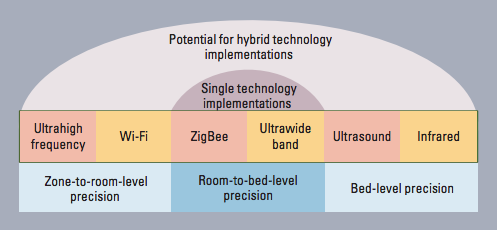
\includegraphics[scale=0.6]{RTLS_tech}}
                \caption{ A comparison of commonly used RTLS technologies used in hospitals \cite{Dsouza2011emergency}}
                \label{fig:litRev_RTLSdirectSensing}
          	  \end{figure}

\begin{comment}
  \begin{table}[ht!]
              \centering
              \caption{RF Technology Comparison}
              \label{tab:litRev_RFcompare}
              \begin{tabular}{l l l p{5cm}}
              \textbf{RTLS technology standard} & \textbf{Frequency/wavelength} & \textbf{Accuracy} & \textbf{Potential interference} \\ \hline \noalign{\smallskip}
              Ultrasound & 35–45 KHz &  & Ultrasonic animal control devices (such as for dogs or birds) \\
              Wi-Fi & 2.4 GHz &  & Wireless LAN (IEEE 802.11b/g), microwave ovens, cordless phones, 2.4 GHz wireless transmitters (audio/video systems, baby monitors) \\ \noalign{\smallskip}
              ZigBee (IEEE 802.15.4) & 2.4 GHz &  & Wireless LAN (IEEE 802.11b/g), microwave ovens,cordless phones, 2.4 GHz wireless transmitters (audio/video systems, baby monitors), temperature sensors \\ \noalign{\smallskip}
              Ultrawide band (UWB) & 2.4 GHz, 6.35–6.67 GHz &  & Aeronautical mobile devices (radar) \\ \noalign{\smallskip}
              Infrared & Approximately 875 nm &  & Remote meter readers, home entertainment remote control systems, automatic door openers (car remotes, garage doors), directed bright light
              \end{tabular}
             \end{table}

\end{comment}         
            
            \subsection{Triangulation}
            A number of systems employ multiple identifiers and triangulation to locate the user. These methods locate the user by triangulating the tags installed in known locations. The tags that have been used for indoor or outdoor localization include RFID, IR, and USID \cite{fallah2013indoor}. As shown in Figure \ref{fig:litRev_triangulation} where $A$ and $B$ represent reference nodes, after obtaining the angles $\theta_1$ , and $\theta_2$ , the physical position of $T$ (representing the target to be located) could then be calculated based on the predetermined coordinates of the reference nodes.
            
            \begin{figure}[htpb!]
                \centering
                \fbox{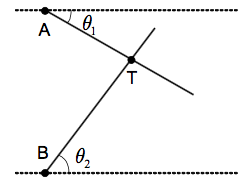
\includegraphics[scale=0.6]{triangulation}}
                \caption{Triangulation-based positioning}
                \label{fig:litRev_triangulation}
          	  \end{figure}
            
            Triangulation based localization methods use the location of at least three known points to determine the users’ location \cite{zheng2010smart}. Lateration uses the distance between the user and at least three known points, whereas angulation uses the angular measurements from at least three known points to the user to determine the users’ location \cite{zheng2010smart}. In the context of indoor areas, where GPS signals are  significantly degraded, the received signal strength (RSS) of either a cell towers or wireless local area network (WLAN) nodes are used to triangulate the position. The precision of the process is generally degraded due to multi-path reflections \cite{fallah2013indoor}. 
            
            \subsection{Pattern-Recognition}
            
            Pattern recognition based localization methods use data from one or more sensors carried or worn by the user and compare this perceived data with set of prior collected raw sensor data that has been coupled with an environment map. This map of sensor data can be created by sampling at different locations or by creating it manually \cite{fallah2013indoor}. Most human navigation systems use a combination of different sensing techniques:
            
            \begin{enumerate}
				\item \textbf{Computer Vision} : While users navigate in an environment, a camera captures images of the environment, and then
by matching the images against a database of images with known location, users’ position and orientation can be determined. The camera captures images while the user navigates \cite{fallah2013indoor}. Using image matching the users’ position and orientation can be determined \cite{fallah2013indoor}. 

The accuracy of camera-based indoor localization systems has reached appreciable levels \cite{mautz2011survey} (i.e., between 10-6 m and 10-1 for high precision systems). Moreover, the increase in both data transmission rate and computational capabilities, as well as the development of high performance image processing algorithm make this technology very efficient. 

A drawback of this technology is that costs are still a bit high but, thanks to the new technologies, low-cost solutions are spreading and recently attention is increasingly directed towards localization systems that use camera-equipped mobile phones \cite{mautz2011survey}. A disadvantage of this technique is the high storage capacity required for storing the images that are coupled with the environment map. Significant computing power may be required to perform the image matching \cite{mautz2011survey}, which may be challenging to implement on a handheld device. Users are often required to carry supporting computing equipment \cite{mautz2011survey}, which may impede their mobility.

                \item \textbf{Fingerprinting} : is the most viable solution for RSS-based indoor localization and works by mapping the observed signal strength of fixed routers placed in the indoor environment into a database (i.e., the radio map) \cite{mainetti2014Indoorlit}. The basic design of the fingerprinting method can be divided in offline stage and online stage. During the offline stage, RSS is collected at sampling locations to build the radio map for the specific environment. During the online stage, the physical location of the client can be estimated by comparing the measured RSS with the stored RSS values \cite{mainetti2014Indoorlit}.
			\end{enumerate}
            
            \subsection{Comparison among technologies} % need to add scalability
            In order to choose the most suitable technology (or a combination of them) for the design and implementation of an indoor localization system, a comparison among the alternative technologies is very useful.
            
             \begin{figure}[htpb!]
             \centering
             \fbox{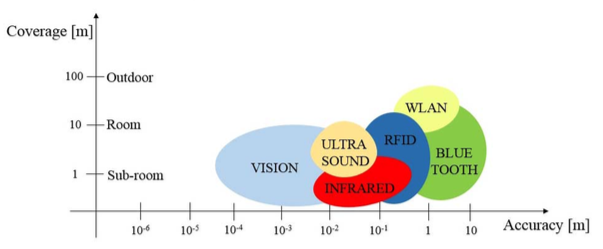
\includegraphics[scale=0.4]{compFig}}
             \caption{Comparison between indoor localisation technologies \cite{mainetti2014Indoorlit}}
             \label{fig:litRev_compFig}
             \end{figure}
            
In Table \ref{tab:litRev_compTable}, some parameters have been selected for the comparison, i.e., accuracy, coverage, cost, complexity, and typical applicative environment. The values of these parameters have a purely indicative meaning as the real values, which depend on many factors, should be evaluated case by case. A graphical overview of all these technologies in dependence of accuracy and coverage is given in Figure \ref{fig:litRev_compFig}. The scalability that many system approaches offer has not been taken into account.

	\begin{table}[htpb!]
		\centering
        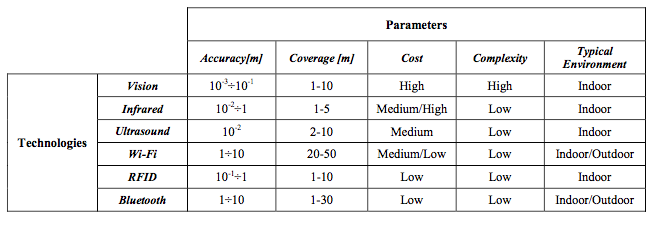
\includegraphics[scale=0.7]{compTable}
        \caption{Comparison between indoor localisation technologies \cite{mainetti2014Indoorlit}}
        \label{tab:litRev_compTable}
	\end{table}

    \section{Social Network Analysis (SNA)} \label{sec:litRev_social}    
    
    	% what is it?
        % where is it used + impact
        % how is it used in infection control + examples
        
        A social network is defined as a social structure of individuals, who are related (directly or indirectly to each other) based on a common relation of interest \cite{sri2008SocialNEt}. SNA is the study of social networks to understand their structure and behavior. Social network analysis has gained prominence due to its use in different applications - from product marketing (e.g. viral marketing) to search engines and organizational dynamics (e.g. management). 
        
        With the aim to identify high risk areas, SNA can play a pivotal role in making use of the mobility data of CF patients. Parameters such as `dwell times', distance between each patient collected from the indoor positioning system can be used to determine high risk areas from cross infection. Specific to infection control, SNA has been applied to the study of infectious disease, including HIV and syphilis in human populations and \textit{Mycobacterium bovis} in captive possums \cite{christley2005infection}. 
     
     % accuracy required from positioning tech